\scanpage{44}
\unsure{XXXXXXXXXXXXXXXXXXXXX}

\deleted{est réduit et \inserted{que les corps composants de} son anneau total des fractions \deleted{est} sont des extensions séparables de $K$. Lorsque $A$ est un anneau de valuation discrète, donc $\widehat A$ également, ces conditions signifient donc aussi que le corps d es fracti-ons $\widehat K$ de $\widehat A$ est une extension séparable de $K$, condition automatiquement satisfaite en particulier si $K$ est de caractéristique nulle.

\figure{\begin{tikzpicture}\node[draw,ellipse] {IV p.224, dans la Bibliographie 36 remplacer Amer. J. par Annals.};\end{tikzpicture}}

\deleted{\uline{IV 8.10.3. supprimer la condition 4º), qui est inutile.}}

\figure{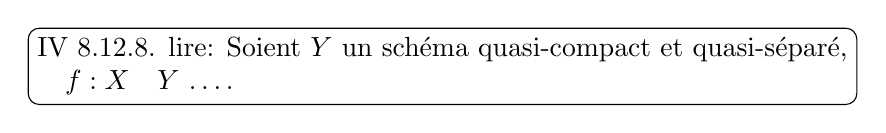
\begin{tikzpicture}\node[draw,rounded corners,align=left] {IV 8.12.8. lire: Soient $Y$ un schéma quasi-compact et quasi-séparé,\\\quad $f:X\quad Y$ $\ldots.$};\end{tikzpicture}}

IV, p.104, l. -10 . au lieu de (17.9.7) lire (17.9.6).

\figure{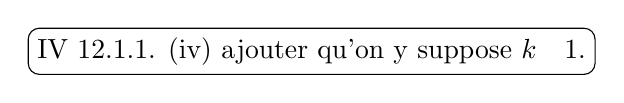
\begin{tikzpicture}\node[draw,rounded corners] {IV 12.1.1. (iv) ajouter qu'on y suppose $k\quad1$.};\end{tikzpicture}}
Ajouter une condition

(vi bis) L(ensemble des $x\quad X$ tels que $\operatorname{prof}^{\bullet}_x(\underline F_{f(x)})\quad k$ .

Dém. La \deleted{condition} question étant locale, on peut supposer $X$ et $Y$ affines, donc $X$ est un sous-schéma fermé d'un $Y\ t_1,\ldots,t_n$, et on est ramené au cas où $X=Y\ t_1,\ldots,t_n$. Utilisant alors (10.8.3) et (\qquad), on trouve que $\operatorname{prof}^{\bullet}_x(\underline F_{f(x)})\quad k$ équivaut à $\text{\uuline{$\operatorname{Ext}$}}^{i}(\underline F_{f(x)},\underline O_{X_{f(x)}})_x=0_x$ pour $i\quad n-k$, et on conclut grâce à (12.3.4) (qui, comme le lecteur le constatera sans surprise, n'utilise pas dans sa démonstration le résul-tat sur la profondeur rectifié qu'on se propose d'établir).
\margin{\unsure{111111111}}

\deleted{\unsure{IV 12.1.4.} \unsure{Ajouter} \unsure{un}}

\deleted{\uline{Corollaire} 12.1.4.1. Soient $f:X\quad Y$ et $\underline F$ comme dans 12.1.1. et soit}

\deleted{IV 14.2.16 p. \unsure{202} lire 14.4.8 a'') L'équivalence de cette propriété \inserted{avec les autres}}

IV 14.4.8. a'')b)Pour formuler ces\deleted{\unsure{t}} hypothèses, il faut supposer que l'ensemble des composantes irréductibles de $Y$ est localement fini.

IV 14.4.10. (i), p.215 l.15 remplacer ``quelconque'' par ``dont l'ensemble des composantes irréductibles est localement fini'', et l.16 remplacer ``type fini'' par ``présentation finie''.
}

\margin{10.9.11.1}
\mspage{43}
